%
% File acl2017.tex
%
%% Based on the style files for ACL-2015, with some improvements
%%  taken from the NAACL-2016 style
%% Based on the style files for ACL-2014, which were, in turn,
%% based on ACL-2013, ACL-2012, ACL-2011, ACL-2010, ACL-IJCNLP-2009,
%% EACL-2009, IJCNLP-2008...
%% Based on the style files for EACL 2006 by 
%%e.agirre@ehu.es or Sergi.Balari@uab.es
%% and that of ACL 08 by Joakim Nivre and Noah Smith

\documentclass[11pt,a4paper]{article}
\usepackage[hyperref]{acl2017}
\usepackage{times}
\usepackage{latexsym}


%for the table
\usepackage{booktabs}

%for [H]
\usepackage{float}
\usepackage{graphicx}
\PassOptionsToPackage{hyphens}{url}\usepackage{hyperref}

\usepackage{url}
\newcommand{\textprime}{\ensuremath{'}}


\aclfinalcopy % Uncomment this line for the final submission
%\def\aclpaperid{***} %  Enter the acl Paper ID here

%\setlength\titlebox{5cm}
% You can expand the titlebox if you need extra space
% to show all the authors. Please do not make the titlebox
% smaller than 5cm (the original size); we will check this
% in the camera-ready version and ask you to change it back.

\newcommand\BibTeX{B{\sc ib}\TeX}

\title{Stock Price Prediction Using Twitter}

\author{Amal Duriseti \\
	 904331855 \\
	% \\
	 \\
	\small{\tt aduriseti@gmail.com } \\\And
	Jonathan Hurwitz \\
	804258351 \\
%	 \\
	 \\
	\small{\tt jdhurwitz@ucla.edu} \\\And
	Fred Xu \\
	004255573 \\
	% \\
	 \\
	\small{\tt xuzeyuanfred@ucla.edu} \\\And
	 Jerry Chen \\
	 804449266 \\
%	 \\
	 \\
	\small{\tt hostmissile@hotmail.com} \\
}
\date{}

\begin{document}
	\maketitle
	\begin{abstract}
	This project aims to predict buy or sell indicators for several large S\&P500 companies based on Twitter data. The first iteration of our project aimed to predict mood based on tweets, but we pivoted and leveraged learnings from the previously done sentiment analysis work in order to build our stock predictor. Several machine learning models have been tested and compared.
	\end{abstract}
	

\section{Introduction}
The former goal was to create an aggregate mood detector and predictor by training machine learning models to perform sentiment analysis on tweets. This task implicitly includes building some method of obtaining more data, such as a data crawler. While our models showed reasonably good performance when trained on the twitter sentiment analysis training corpus\footnote{The sentiment analysis corpus contains 1.5M tweets and can be downloaded at \url{http://thinknook.com/twitter-sentiment-analysis-training-corpus-dataset-2012-09-22/}}, we realized that some sort of unsupervised learning would have to be done in order to label future data obtained via the crawler. This motivated us to explore other ways in which we could leverage our previous work but for a task with an easier means of labeling data.
\par
Using sentiment to predict buy or sell indicators seemed like a natural progression with an easier way of labeling data. The labeling scheme we chose was to associate each tweet with the corresponding stock price on the day it was tweeted. The crawler pulls tweets and labels each tweet by doing a yahoo finance price lookup. This way, we are able to build an arbitrarily large dataset of labeled tweets in order to better train our models. There is no need for unsupervised learning such as clustering in order to assign class labels.
\par
All code for this project can be found here: \url{https://github.com/aduriseti/cs145_project}
\section{Data Crawler}
The data crawler performs tweet lookup, preprocessing, and labeling for an arbitrary number of stock tickers or query strings. It is assumed that data for each query will be pulled for each day within the specified date range. 
\par
Within the scope of this project, the queries were all stock tickers for several large companies: AAPL, AMZN, SNE, GOOG, NVDA, INTC, HPQ, MSFT, IBM, and TXN. Each of these tickers is given their own thread to perform the lookup, filtering, and labeling. The initial intent was to perform a live lookup on Yahoo finance in order to obtain stock prices for labeling, but there were issues with Yahoo finance historical data. After writing a function to pull data using BeautifulSoup, we decided it would be best to just download local csv files from Yahoo containing the data for each ticker over the desired time range (from min to max date). 
\par 
For each day in the date range, the crawler queries twitter and limits the number of tweets pulled via the "max\_tweets" parameter.  Tweets are processed in batches corresponding to each day. Tweets for a specific ticker that were posted on a day in which there is no associated stock price are removed from the set. Duplicates are also removed. Stock price labels are 5-D and consist of the open, high, low, close, and adj close. The intent was to provide the maximum amount of information for us to use in learning algorithm evaluation. Following a successful tweet:label pairing, the crawler writes this to a file along with the date of the tweet and continues.

\section{Sentiment Analysis}
We trained a variety of classifiers on the Twitter sentiment analysis training corpus. These included random forest, multi-layer perceptron (MLP), and quadratic discriminant analysis. In addition, we tested the RNN-based long short-term memory (LSTM) model. SVM was avoided due to long training time. Metrics used to judge performance include accuracy, precision, recall, and F1 score. 
\par
The embedding scheme involved using word2vec and a mean aggregation method. The word2vec vectors are trained on the set of aggregated tweets created by the crawler. For each word within a tweet, we check to see if it is in the trained word2vec model. If so, the word2vec vector corresponding to that word gets added to a running sum for the tweet. If a word does not appear in the word2vec model, then it is zero padded. After all the words have been checked, this summed vector is divided element-wise by the number of words in the tweet in order to obtain a mean vector. This is a form of summarization. 
\par
The word2vec model is using dimension 100 vectors, and the resulting summarized tweet vectors are also of dimension 100.
\subsection{Random Forest}
Random forest provided the initial baseline:
\begin{table}[h!]
	\begin{center}
		\caption{word2vec + Random Forest Classifier}
		\label{tab:table1}
		\begin{tabular}{l|c|r} % <-- Alignments: 1st column left, 2nd middle and 3rd right, with vertical lines in between
			\textbf{Type} & \textbf{Training Set} & \textbf{Test Set}\\
			\hline
			Accuracy & 0.684591533095 & 0.673612152101 \\
			Precision & 0.681912795793 & 0.67805020432 \\
			Recall & 0.82712112152  & 0.821646476258\\
			F1 score & 0.750909267723 & 0.73868361183
		\end{tabular}
	\end{center}
\end{table}


\begin{figure}[H]
	%\hspace*{-1.85cm}
	\centering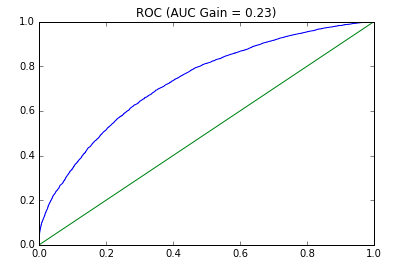
\includegraphics[scale=0.55]{ROC_rf} 
	\caption{\textbf{Figure 1: Random forest classifier ROC with AUC Gain=0.23 }}
\end{figure}


\begin{figure}[H]
	%\hspace*{-1.85cm}
	\centering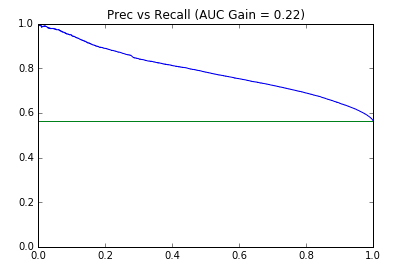
\includegraphics[scale=0.55]{prrc_rf} 
	\caption{\textbf{Figure 2: Random forest classifer precision vs. recall with AUC Gain=0.22 }}
\end{figure}

\subsection{Multi-Layer Perceptron}
MLP yielded better accuracy on both training and test sets compared to random forest:
\begin{table}[h!]
	\begin{center}
		\caption{word2vec + MultiLayer Perceptron (MLP)}
		\label{tab:table1}
		\begin{tabular}{l|c|r} % <-- Alignments: 1st column left, 2nd middle and 3rd right, with vertical lines in between
			\textbf{Type} & \textbf{Training Set} & \textbf{Test Set}\\
			\hline
			Accuracy & 0.811256993379 & 0.742028552952 \\
			Precision & 0.828856719281 & 0.765130190007 \\
			Recall & 0.840213932107  & 0.775637595862\\
			F1 score & 0.834496685544 & 0.77034806483
		\end{tabular}
	\end{center}
\end{table}


\begin{figure}[H]
	%\hspace*{-1.85cm}
	\centering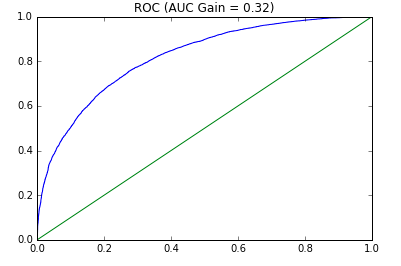
\includegraphics[scale=0.55]{ROC_nn} 
	\caption{\textbf{Figure 3: MLP classifier ROC with AUC gain=0.32 }}
\end{figure}


\begin{figure}[H]
	%\hspace*{-1.85cm}
	\centering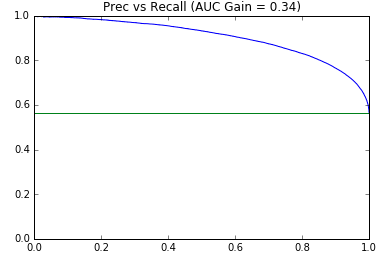
\includegraphics[scale=0.55]{prrc_nn} 
	\caption{\textbf{Figure 4: MLP classifier precision vs. recall with AUC Gain=0.34 }}
\end{figure}

\subsection{Quadratic Discriminant Analysis}
QDA is a Bayesian classifier. Training and test accuracies were better than the baseline random forest but not as high as the multilayer perceptron classifier. 
\begin{table}[h!]
	\begin{center}
		\caption{word2vec + Quadratic Discriminant Analysis}
		\label{tab:table1}
		\begin{tabular}{l|c|r} % <-- Alignments: 1st column left, 2nd middle and 3rd right, with vertical lines in between
			\textbf{Type} & \textbf{Training Set} & \textbf{Test Set}\\
			\hline
			Accuracy & 0.719376196853 & 0.71173456698 \\
			Precision & 0.769485042382 & 0.760003838403 \\
			Recall & 0.720252828854  & 0.706260032103\\
			F1 score & 0.744055433157 & 0.732146984054
		\end{tabular}
	\end{center}
\end{table}

\begin{figure}[H]
	%\hspace*{-1.85cm}
	\centering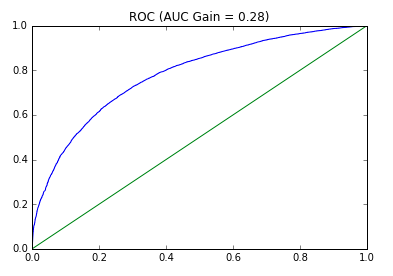
\includegraphics[scale=0.55]{ROC_qda} 
	\caption{\textbf{Figure 5: QDA classifier ROC with AUC gain=0.28 }}
\end{figure}


\begin{figure}[H]
	%\hspace*{-1.85cm}
	\centering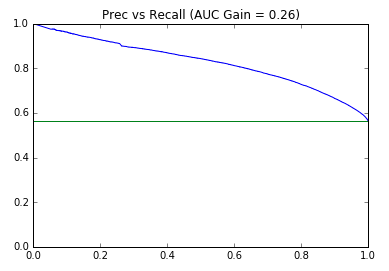
\includegraphics[scale=0.55]{prrc_qda} 
	\caption{\textbf{Figure 6: QDA classifier precision vs. recall with AUC Gain=0.26 }}
\end{figure}


\subsection{LSTM}
The LSTM has a notion of memory. Its memory cell consists of four main elements: an input gate, a neuron with a path back to itself, a forget gate, and an output gate. The loop back allows the state of a memory cell to remain constant through time. The forget gate modulates the loop back and can allow the cell to “delete” or “forget” its previous state. LSTMs do not suffer from the vanishing or exploding gradient problem when long sequences are processed. It is an effective model for data that exhibits long-chain dependencies.  
\subsubsection{LSTM Architecture}
\begin{figure}[H]
	%	\hspace*{-1.3cm}
	\centering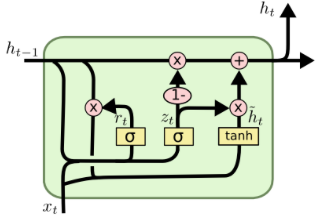
\includegraphics[scale=0.5]{lstm_image} 
	\caption{\textbf{ LSTM architecture.}}
\end{figure}

The figure above shows the basic LSTM architecture, including the notion of time (t-1 is introduced) and the gates previously discussed. Corresponding functions are shown below.
\begin{figure}[H]
	%	\hspace*{-1.3cm}
	\centering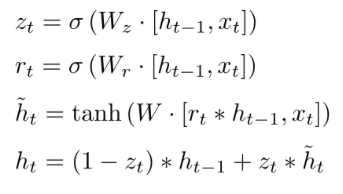
\includegraphics[scale=0.5]{lstm_functions} 
	\caption{\textbf{ LSTM functions.}}
\end{figure}

Our specific network's architecture consists of three layers. Words will be fed into the word embedding layer, which will map words to word embeddings. The resulting word vectors are passed into LSTM cells, whose output will be passed into a dense layer with softmax activation function, and makes a prediction.
\begin{figure}[H]
	%	\hspace*{-1.3cm}
	\centering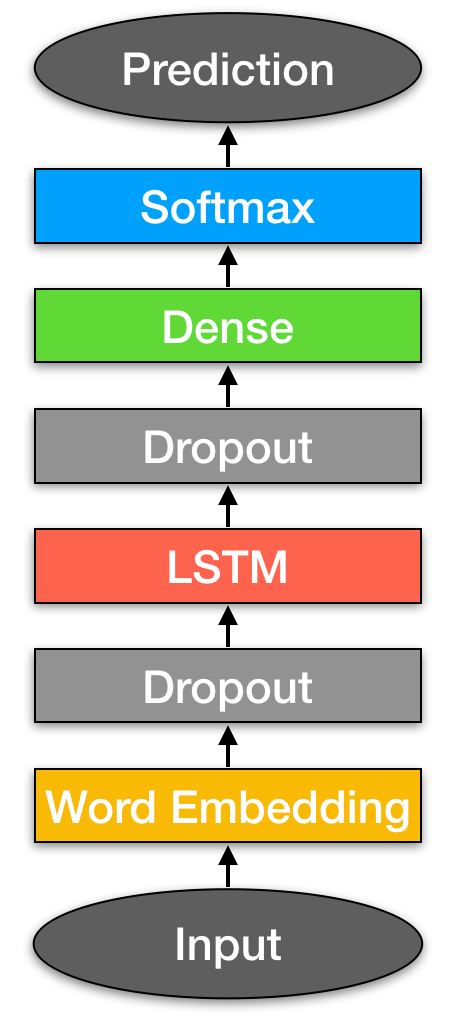
\includegraphics[scale=0.3]{architecture} 
	\caption{\textbf{ LSTM implementation architecture.}}
\end{figure}

\subsubsection{LSTM Implementation}
Our LSTM model is implemented with Keras, running on top of TensorFlow. Keras is a high-level neural network API, which allowed us to quickly implement the model by simply stacking layers together:
{\tt \small
	\begin{verbatim}
	model = Sequential()
	model.add(Embedding(...))
	model.add(Dropout(...))
	model.add(LSTM(...))
	model.add(Dense(..., activation='softmax'))
	\end{verbatim}
}

Our work largely follows Peter Nagy's implementation\cite{peter}, but we modified the network and tuned hyperparameters to suit our needs. Training the model took two hours to finish.

\subsubsection{LSTM Results}
The model achieves an F1-score of 0.81 and an Accuracy of 0.81 on test datasets, outperforming the first classifier's F1-score of 0.78 and Accuracy of 0.75.  \\
%TODO verify max classifier performance

\begin{center}
	\begin{tabular}{|c|c|}
		
		\hline
		Metrics & Value \\
		\hline
		Accuracy & 0.810448419184 \\
		Precision & 0.803874201171 \\
		Recall & 0.822235970902 \\
		F1-score & 0.812951416989 \\
		\hline
	\end{tabular}
\end{center}



\section{Stock Prediction} 


\section{Hyperparameter Tuning}
The hyperparameter tuning targets the hyperparameters of the word2vec model. Cross-validation was used on the original dataset. Since the MLP classifier had the best performance during the sentiment analysis evaluation phase, we chose to use this is the go-to classifier and invariant pairing. The F1-score of the word2vec + MLP classifier is used as a performance metric. Higher F1 score indicates a better performance. 
\subsection{Testing Methodology}
Word2vec turns text messages into word vectors. However, there is no systematic metric for the evaluation of the model alone. Therefore, evaluation of the bundle: Word2vec + MLP, was used to test the performance. \par
The default method for hyperparameter tuning is to use an exhaustive grid search. However, since a single run of the 5-fold cross validation takes around 50 minutes, and some hyperparameters, such as size and iter, change the amount of work to be done, a brute force method would be too time consuming. Therefore hyperparameter selection and candidate selection was used. In the selection part, several hyperparameters are examined and the relatively important ones are picked. The resulting candidates for the tuning are:
\begin{itemize}
	\item Size, which determines the dimensionality of the feature vector.
	\item \texttt{wind\_size}, the maximum distance between current and predicted words within a sentence, governs the context of words.
	\item \texttt{min\_count}, which defines the cut-off threshold for words.
	\item iter, number of iterations over the corpus.
\end{itemize}
The candidates for size is picked in the range from the default 100 to 150, \texttt{wind\_size} is picked from 1 to 10, which includes its default value 5. \texttt{min\_count} and iter are similar to the \texttt{wind\_size}. 
\par
This means a 2-D grid search could take around 3000 testing instances, which is impossible to handle. Therefore, 1-D search was performed on each hyperparameter, and a final search in the potential best candidate's neighborhood was conducted.
\par
The final candidates were further reduced based on their the neighbor's frequency in the 1-D search. If one of the two neighbors in the 1-D case has significantly lower score, it is omitted. Furthermore, size values are limited to only multiple of 4 to improve performance.

\subsection{Testing Results}
The following table summaries the 1-D search and the resulting search. 
%\hspace{-1cm}
\begin{tabular}{|c|c|c|c|}
	\hline 
	hyperparameter & optimum F1 & best value & candidate \\
	\hline 
	\texttt{wind\_size} &  0.6286 & 1 & 1,4\\ 
	\hline 
	size & 0.657 & 130, 140  & 132, 140 \\
	\hline 
	\texttt{min\_count} & 0.6026 & 7 & 7,8 \\
	\hline 
	iter & 0.6101 & 9 & 9, 10 \\
	\hline 
\end{tabular}
The neighborhood search in the end gives the best candidates for hyperparameters: (140,1,7,9), (140,1,8,9), (140,1,8,10), and (140,4,8,10).

\section{Discussion}

\subsection{Future Work}
Due to time limitations, we were not able to integrate the trained LSTM model with the rest of our functional blocks. However, our design was pipelined such that blocks (preprocessor, embedding scheme, sentiment analysis, and prediction) can be easily interchanged. 
% include your own bib file like this:
%\bibliographystyle{acl}
%\bibliography{acl2017}
%\nocite{*}
%\bibliography{fr_bib}
%\bibliographystyle{acl_natbib}



\appendix


	
\end{document}
